\section{Lezione 17 - Clustering}\label{lezione-17---clustering}

Il clustering è il processo che partiziona un'insieme di oggetti in
sottogruppi in modo che gli oggetti di questi gruppi siano simili tra
loro.

Questa tipologia di apprendimento prende il nome di
\textbf{apprendimento non supervisionato} dal momento che  non c'è un supervisore che fornisce delle etichette per i dati di apprendimento.

\subsection{Il problema del clustering}\label{il-problema-del-clustering}

Tipicamente è composto da:

\begin{itemize}
\item
  Un insieme di esempi, detti anche documenti $D = \{d_1, \ldots , d_n\}$
\item
  Una misura di similarità o distanza, decisa da noi
\item
  Un criterio di partizionamento
\item
  Un numero desiderato di cluster \emph{K}.
\end{itemize}

L'algoritmo di clustering calcola quindi una funzione di assegnamento $\gamma$
che prende un elemento di \emph{D} e lo assegna ad un gruppo
$\{1, \ldots , K\}$, in modo che non ci siano cluster vuoti, secondo un certo criterio, come la misura di similarità.

\subsection{Problemi del clustering}\label{problemi-del-clustering}

Come rappresentare i dati? Anche in questo caso è necessario utilizzare
una rappresentazione nel vector space, normalizzando i dati. Inoltre, la
rappresentazione influisce sulla misura di similarità.

Serve poi una notazione per la similarità/distanza.

C'è anche il problema di quanti cluster fare, se stabilirlo a priori o
sceglierlo in base ai dati, evitando i casi triviali con cluster troppo
grandi o troppo piccoli.

\subsection{Funzione obiettivo}\label{funzione-obiettivo}

Tipicamente l'obiettivo di un problema di clustering è quello di
ottimizzare una funzione, definendo così un problema di ricerca tra i
possibili assegnamenti.

Questi stati sono tanti, $\frac{K^N}{K!}$. Il \emph{K!} serve per togliere i
cluster equivalenti, cioè quando la divisione degli elementi è identica
ma cambia ``l'etichetta'' dei cluster a cui sono assegnati.

Tra l'altro ci sono dei problemi con i minimi locali per la funzione
obiettivo, possono essercene tanti e possono impedire di raggiungere un
minimo ottimo.

\subsection{Valutazione di un clustering}\label{valutazione-di-un-clustering}

Ci sono dei \textbf{criteri interni} che vanno a misurare la similarità
tra oggetti della stessa classe (\textbf{intra-class}) e tra oggetti di
classi diversi (\textbf{inter-class}), un buon clustering cerca quindi
di massimizzare l'intra-class e di minimizzare l'inter-class.

La qualità misurata inoltre dipende da come vengono rappresentati i dati
e dalla misura di similarità adottata.

Ci sono poi i \textbf{criteri esterni} che misurano la capacità dell'algoritmo nel trovare dei pattern tra i dati, ad esempio confrontando i cluster prodotti rispetto ad un partizionamento noto che prende  il nome di \textbf{ground truth}.

Si assume quindi che i documenti possano essere partizionati in \emph{C}
classi che rappresentano la ground truth e che l'algoritmo di clustering
produca \emph{K} cluster, $\omega_1, \ldots, \omega_K$, ognuno contenente
$n_i$ documenti.

La misura più semplice prende il nome di \textbf{purity} e rappresenta
il rapporto medio tra i vari cluster che c'è tra la classe nominante $\pi_i$in
quel cluster e la dimensione del cluster $\omega_i$.

Altre misure si basano sull'entropia.

\begin{figure}[htbp]
\centering
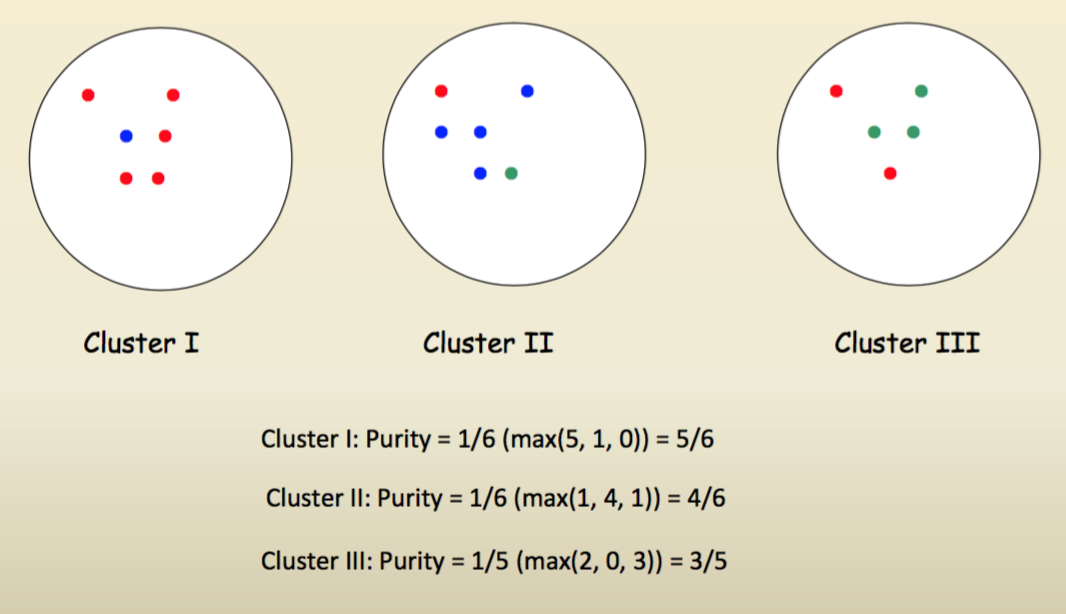
\includegraphics[width=\textwidth]{./notes/immagini/l17-purity.png}
\caption{Purity calcolata su 3 cluster}
\end{figure}

Nell'esempio il numero di cluster coincide con il numero di etichette ed è
una cosa voluta, ma il gioco funziona anche con un numero diverso di
cluster.

Questo perché le etichette note a priori vengono utilizzate solamente per valutare il clustering e non per effettuare l'apprendimento.

\subsubsection{Rand Index}\label{rand-index}

È una misura di similarità tra cluster, definita come il rapporto tra il
numero di elementi che hanno la stessa classe ground e si trovano nello
stesso cluster e con classi diverse in cluster diversi, sul numero
totale di elementi.

In altre parole è il rapporto tra il numero di elementi che si trovano nel cluster corretto e il numero totale di elementi.

\begin{figure}[htbp]
\centering
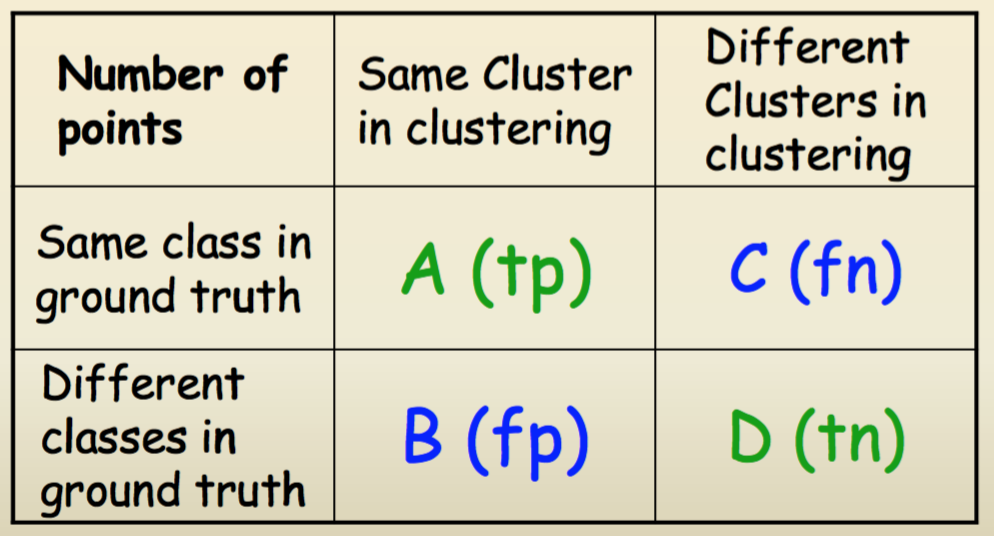
\includegraphics[width=0.6\textwidth]{./notes/immagini/l17-rand-index.png}
\caption{Elementi necessari per il Rand Index}
\end{figure}

Per calcolare il Rand Index, viene creata una tabella di contingenza, valutando per ogni coppia di
punti, se hanno etichette diverse e se sono nello stesso cluster.

Probabilmente, ma non ne sono sicuro, i numeri della tabella corrispondo
alle coppie che rispondo a quella categoria.

In questo modo ci si riconduce all'accuracy:

$$
RI =\frac{A + D}{A+B+C+D}
$$

Allo stesso modo si possono calcolare \textbf{precision} e
\textbf{recall} (§\ref{sec:pre-rec})

$$
P = \frac{A}{A+B} \qquad R = \frac{A}{A+C}
$$

\subsection{Algoritmi di Clustering}\label{algoritmi-di-clustering}

Ci sono due tipologie di algoritmi:

\begin{itemize}
\item
  \textbf{partitional}: che partono da un partizionamento casuale e
  cercano di migliorarlo iterativamente (K-means clustering, Model based
  clustering)
\item
  \textbf{hierarchical}: che vanno a definire un clustering come un
  albero in cui la radice contiene tutti gli esempi e man mano che si
  scende questi vengono partizionati. Si può usare un approccio
  \textbf{agglomerative} che costruisce l'albero in modo bottom-up
  (permettendo di fissare un numero di cluster), o \textbf{divisive} che
  funziona in top-down, applicando K-means sulla radice e poi
  ricorsivamente su ogni figlio, arrivando fino alla foglie che
  consistono in cluster di un solo elemento.
\end{itemize}

\subsection{K-means}\label{k-means}

Questo algoritmo appartiene alla categoria degli algoritmi di
partizionamento, ovvero vengono partizionati gli \emph{n} documenti in
\emph{K} cluster, cercando di trovare un partizionamento ottimo secondo
un determinato criterio.

Gli elementi da clusterizzare sono dei vettori con numeri reali e come
criterio di partizionamento si utilizza la distanza vettoriale tra gli
esempi e il centro del cluster.

Si cerca quindi di creare dei cluster che minimizzano il raggio della
iper-sfera che contiene gli esempi e che ha come centro $c$. (cluster \textbf{centroidi})

La formula da minimizzare è la seguente:

$$
\vec{\mu}(c) = \frac{1}{|c|}\sum_{\vec{x} \in c} \vec{x}
$$

\subsubsection{Algoritmo}\label{algoritmo}

\begin{enumerate}
\item
  Si posizionano K punti a caso nello spazio degli oggetti da
  clusterizzare, questi punti rappresentano i centroidi dei cluster.
\item
  Si assegna ogni oggetto al centroide più vicino.
\item
  Una volta completato l'assegnamento si ricalcola la posizione di tutti
  i centroidi utilizzano la media dei valori di tutti gli oggetti che
  sono finiti nel cluster.
\item
  Si ripetono i passi 2 e 3 finché non si spostano più i centrodi, ovvero finché non si raggiunge un punto fisso.
\end{enumerate}

L'iper-parametro $K$ dell'algoritmo è tipicamente soggetto a dei vincoli noti a priori oppure è da ottimizzare, ovvero trovare il numero \textit{corretto} di cluster in cui si dividono i dati.

\subsection{Approcci gerarchici agglomerativi}\label{approcci-gerarchici-agglormerativi}

\textbf{quelli divisi utilizzano ricorsivamente k-means}

Costruiscono un dendogramma a partire dagli oggetti, che vengono
agglomerati tra loro quando vengono trovati simili. Si ripete il
procedimento finché tutti gli oggetti non vengono agglomerati in un
unico cluster.

Si parte quindi da \textit{N} cluster, uno per ogni esempio e si agglomerano via
via finché non si ottiene un unico cluster.

Ad ogni iterazione l'algoritmo può essere interrotto per evitare di
ottenere un unico cluster.

Le linee verticale di un dendogramma rappresentano un cluster, mentre
quelle orizzontali rappresentano un punto di \textbf{merge} ovvero
quando la similarità di due cluster è tale che vengono uniti in un unico
cluster.

\begin{figure}[htbp]
\centering
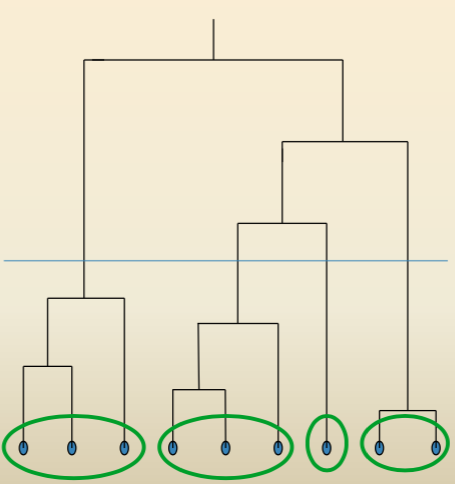
\includegraphics[width=.5\textwidth]{./notes/immagini/l17-clustering.png}
\caption{Esempio di un dendogramma}
\end{figure}

In base alla misura di similarità l'operazione può essere
\textbf{monotona} o meno, cioè se $s_1, \ldots, s_{k-1}$ sono
combinazioni di similarità associate a delle operazioni di merge, allora
$s_1 \geq s_2 \geq \ldots \geq s_{k-1}$

La non monotonicità, ovvero l'aumento della similarità in una serie di merge, contraddice l'assunzione fondamentale che cluster con pochi elementi sono più coerenti di cluster con tanti elementi\footnote{\url{http://nlp.stanford.edu/IR-book/html/htmledition/centroid-clustering-1.html}}.

\subsubsection{HAC - Hierarchical agglormerative
Clustering}\label{hac---hierarchical-agglormerative-clustering}

Prima viene creato un cluster per ogni esempio, dopodiché viene eseguito
via via il merge del \textbf{closest pair}, ovvero dei due cluster più
simili, fino a che non rimane un unico cluster. Lo storico dei merge
crea il dendogramma.

Come criteri di similarità tra i due cluster è possibile utilizzare:

\begin{itemize}
	\item la distanza euclidea: $||a-b||^2$, più è bassa, più simili sono i cluster
	\item la similarità coseno: $\frac{A \cdot B}{||A|| \cdot ||B||}$ che tende a 1 se i due esempi sono simili e a 0 se sono diversi.
	\item distanza di Manhattan: $\sum_i|a_i - b_i|$, più è bassa, più simili sono i cluster
\end{itemize}

Una volta scelta la misura di similarità, questa può essere calcolata per una coppia di cluster in vari modi:

\begin{itemize}
\item
  \textbf{single link}: viene calcolata la similiarità tra tutti gli elementi dei due cluster e viene scelto il valore massimo.
\item
  \textbf{complete link}: viene calcolata la similarità tra tutti gli elementi dei due cluster e viene scelto il valore minimo
\item
  \textbf{centroid link}: viene utilizzata la similarità tra i due centroidi dei due cluster
\item
  \textbf{average link}: viene calcolata la similarità tra tutti gli elementi dei due cluster e ne viene fatta la media.
\end{itemize}

Single, complete e average link garantiscono la monotonicità, mentre utilizzando centroid link alcune operazioni di merge potrebbero essere non monotone, ad esempio quando è necessario fare il merge di 3 cluster equidistanti tra loro.

Una volta calcolata la similarità tra tutti i cluster viene scelto il closest pair e viene fatto il merge.

\paragraph{Esempio - Distanza euclidea}

Scegliendo come misura la distanza euclidea, si ottiene che \textbf{minore è la distanza, più simili sono i cluster}. Pertanto i vari modi per calcolarle la similarità diventano:

\begin{itemize}
	\item
	\textbf{single link}: distanza tra i due punti più vicini dei due cluster
	\item
	\textbf{complete link}: distanza tra i due punti più lontani dei due cluster
	\item
	\textbf{centroid link}: distanza tra i centroidi dei due cluster
	\item
	\textbf{average link}: distanza media tra tutti i punti dei due cluster
\end{itemize}

\paragraph{Esempio - Similarità coseno}

Scegliendo come misura la similarità coseno, si ottiene che \textbf{maggiore è il valore, più simili sono i cluster}. Pertanto i vari modi per calcolarle la similarità diventano:

\begin{itemize}
	\item
	\textbf{single link}: similarità coseno tra i due punti più simili dei due cluster, ovvero che hanno similarità coseno più vicina ad 1.
	\item
	\textbf{complete link}: similarità cosento tra i due punti più diversi dei due cluster, ovvero che hanno similarità coseno più vicina a 0.
	\item
	\textbf{centroid link}: similarità coseno tra i due centroidi dei cluster
	\item
	\textbf{average link}: similarità media tra tutti gli elementi dei 
\end{itemize}

\begin{figure}[htbp]
\centering
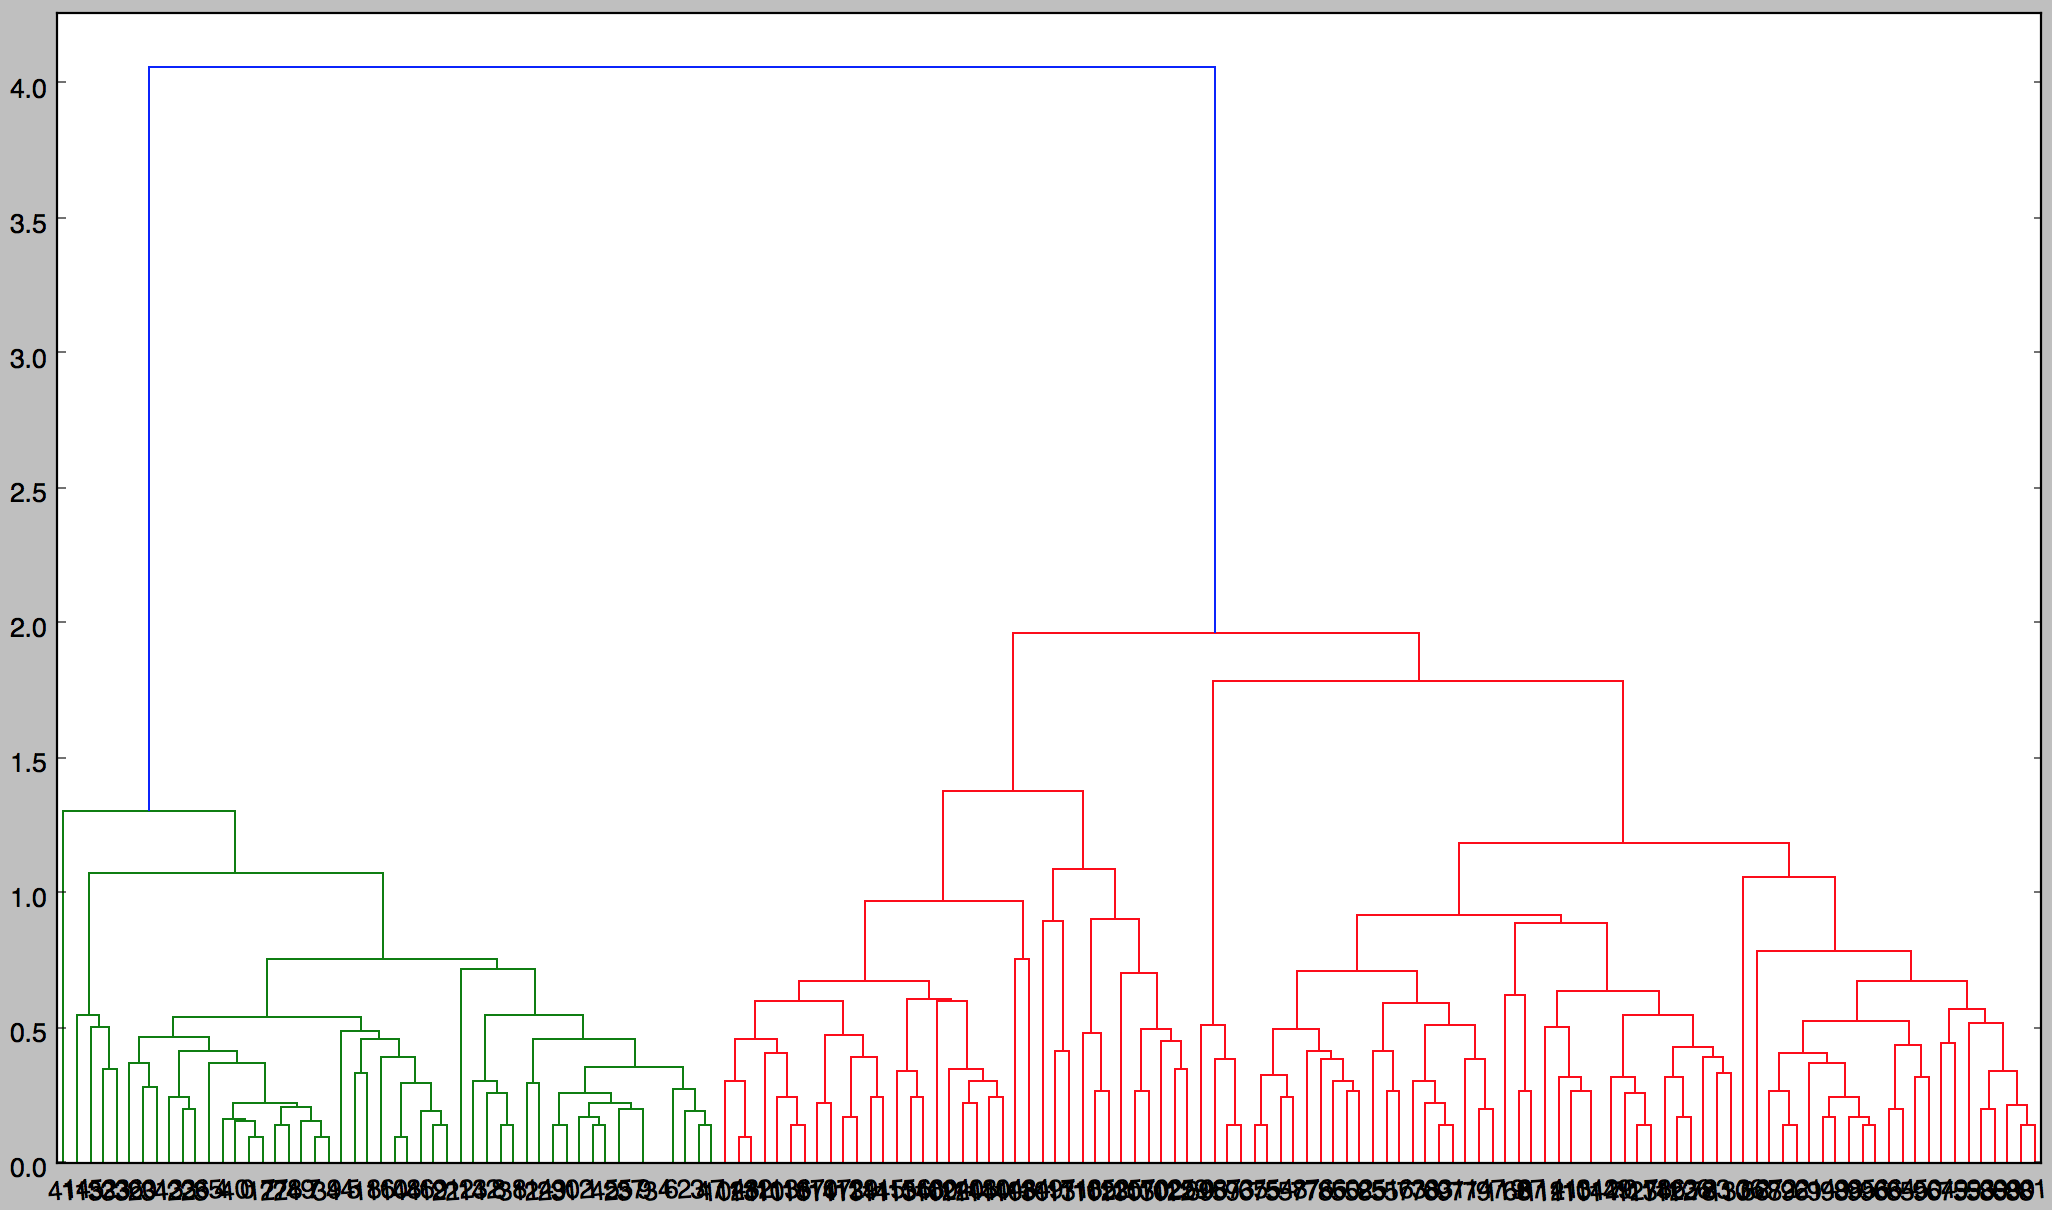
\includegraphics[width=\textwidth]{./notes/immagini/l17-dendogram-cluster.png}
\caption{Esempio di clustering ottenuto con HAC}
\end{figure}

Sia single link che complete link garantiscono la monotonia, tuttavia
con single link si tendono a creare dei cluster che sono delle
\emph{catene}, ovvero si ottengono dei dendogrammi sbilanciati, mentre
il complete link tende a dare dei cluster sferici e più compatti, se
però ci sono degli esempi \textbf{outliers}\todo{Da verificare}, ovvero che escono dalla
distribuzione.

Il centroid link è carino ma non garantisce la monotonia.

\begin{figure}[htbp]
\centering
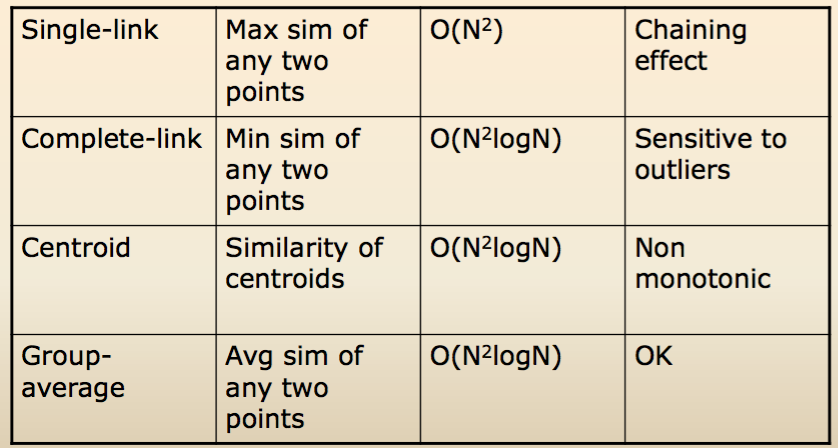
\includegraphics[width=\textwidth]{./notes/immagini/l17-riassunto.png}
\caption{Tabella riassuntiva, le complessità della tabella indicano quante operazioni servono per
	scegliere il closest pair}
\end{figure}
